\section{Data Provenance Model}
In this section, we shortly explain some of the existing provenance data models and the need for a new data model, then we explain a new data model\footnote{\url{https://link.springer.com/content/pdf/10.1007\%2F978-3-319-68136-8.pdf}} specialized in the IoT context.
\lstset{stringstyle=\color{black}}

\subsection{Existing Data Models}
As of today, there is no standard way to represent provenance information. Existing approaches for modeling data provenance include the Open Provenance Model\footnote{\url{http://www.opmw.org/model/OPMW/}} (OPM) and the Provenance Data Model\footnote{\url{https://www.w3.org/TR/prov-dm/}} (PROV-DM).

\subsubsection {Open Provenance Model}
The Open Provenance Model is designed to allow provenance information to be exchanged between systems, by means of a compatibility layer based on a shared provenance model. The Open Provenance Model offers several core concepts and relationships to represent provenance. It models the resources (datasets) as artifacts (immutable pieces of state), processes (action or series of actions performed on artifacts), and agents (controllers of processes). Their relationships are modeled in a provenance graph with five causal edges.

\subsubsection {PROV-DM}
PROV-DM is a refinement of OPM and aims at covering a broader range of application domains than OPM. It is structured in six components, dealing with: 

\begin{enumerate}
	\item Entities and activities, and the time at which they were created, used, or ended.
	\item Agents bearing responsibility for entities that were generated and activities that happened.
	\item Derivations of entities from entities.
	\item Properties to link entities that refer to the same thing.
	\item Collections forming a logical structure for its members.
	\item A simple annotation mechanism.
\end{enumerate}

\subsection{Need for new Data Model}
OPM and PROV-DM are quite generic and adopt a largely document-centric view that is centered on expressing actions performed on documents and the causal relationships between such actions while data provenance for IoT systems requires more focus on data exchanged.

\subsection{New Data Model}

We define a data point (DP) as a uniquely identifiable and addressable piece of data (i.e., a value) in the context of the smart grid. Examples for DPs in the context of smart grid includes sensor readings such as 3-phase electric currents, complex analytics results derived from sensor readings etc. The unique identifier is composed of three blocks.
\begin{itemize}
	\item Unique Identifier - A data point distinguishes itself specifically from other data flowing in the Data Provenance Model for smart grid  (e.g., bulk sensor readings that are of no further interest, ephemeral intermediary analytics results, etc.) in that it is addressable, i.e., it has an ID that is unique in the context of the smart grid. In order to ensure the uniqueness of the identifier, we came up with an identifier generation strategy, which generates a unique ten-byte identifier and ensures uniqueness across the system. Data point identifier comprised of:
		
		\begin{itemize}
			\item 3-byte node identifier - Guarantees its uniqueness across machines/nodes and processes.
			\item 4-byte value representing the seconds since the Unix epoch - Ensures uniqueness in relation to a single second.
			\item 3-byte counter - Provides uniqueness within a single second in a single process.
		\end{itemize}
		
		\subsection* {Properties} Our unique identifier generation  mechanism along with its simplicity brought some other advantages and reduced the need to store machine/node identifier separately and also ease some time-based queries (e.g., sorting based on generation timestamp).
			\begin{itemize}				
				\item Example: 5a7b91370003c6badfb2
			\end{itemize}
	\item Input Data Points - A data point may be based on other data points that have contributed to its creation or modification. We refer to these related
data points as input data points(IDP). A data point's IDP is a list of unique identifiers of all those data points, which contributed to its creation or transformation. It also stores information about the contribution type.
	
	\begin{itemize}			
			\item Example: 
\begin{lstlisting}			
[{
    "average": [   // Contribution type
        "5a81c07800031ddaf123",
        "5a81c093000a1d341fab"
    ]
}]		
\end{lstlisting}
	\end{itemize}
	\item Context - Specific context for provenance may vary for different IoT applications. We propose a data model for the context of typical IoT environments comprising the concepts of Agents, Execution Context, as well as Time and Location information (cf. \ref{dataModelContext}). An Agent is an entity that creates and/or modifies data points (e.g., sensor, device,  software agent, etc.). It is recursively defined in such a way that an agent can contain other agents (e.g., a device containing several sensors). This recursion allows for defining agents in a hierarchy and may be used as fine-grained as required. For instance, an agent hierarchy may span from the concept of a particular function in a software library running over a virtualization container on a particular device to a particular IoT network. Execution Context provides information related to the provenance event at runtimes, such as events or data points that triggered the creation/modification of the data point. Time and Location information is also added to the provenance information.
\begin{figure}[h]
\centering
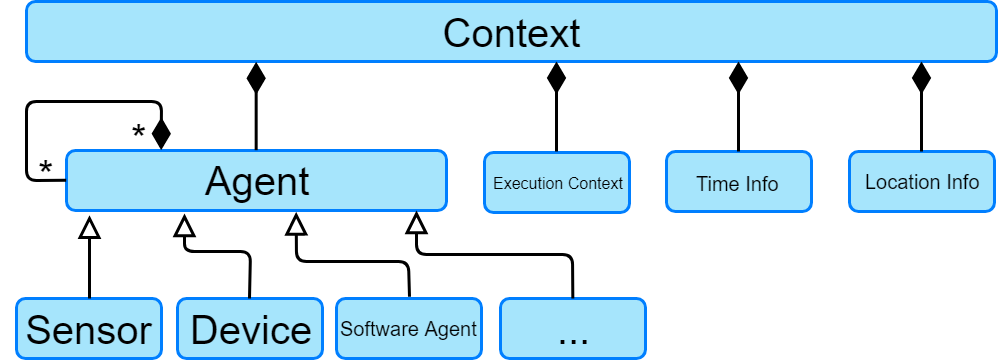
\includegraphics[width=\linewidth]{figures/context.png}\\
\caption{Data Model Context}
\label{dataModelContext}
\end{figure}
We chose two to three specific metrics for each of the above-mentioned context parameters based on our use-cases and these metrics are listed below  (cf. \ref{idpDataModelContext}):
		\begin{itemize}
			\item Node/Machine  identifier - An identity of the physical node.
			\item Creation time - In the case when a node is performing some aggregation and not simply forwarding data values, creation time is the time when that data value is generated.
			\item Send time - Time, when a particular data value is forwarded to next nodes.
			\item Receive time - Time, when a particular data value is received/captured from the previous node or from the sensor.
			\item Application name - An application which is responsible for the creation of data value.
			\item Class name - A class which is responsible for the creation of data value.
			\item Location - The physical location of the node, where a data value got created.
			\item Line of code - The line number of the code that generated a particular data value.
			\item health status
				\begin{itemize}
					\item Node/Machine
					\item Channel
					\item Provenance Daemon
					\item Pipeline Daemon
				\end{itemize}		
		\end{itemize}
We categorize these metrics into two main categories: core metrics and use-case specific metrics. Node/Machine identifier, Creation time, Send time, Receive time and Location are the core metrics of our provenance system. All other metrics are use-case specific: Application name, class name and code line number are for debugging and tracing use-case while health status is for error detection use-case.

\begin{figure}[h]
\centering
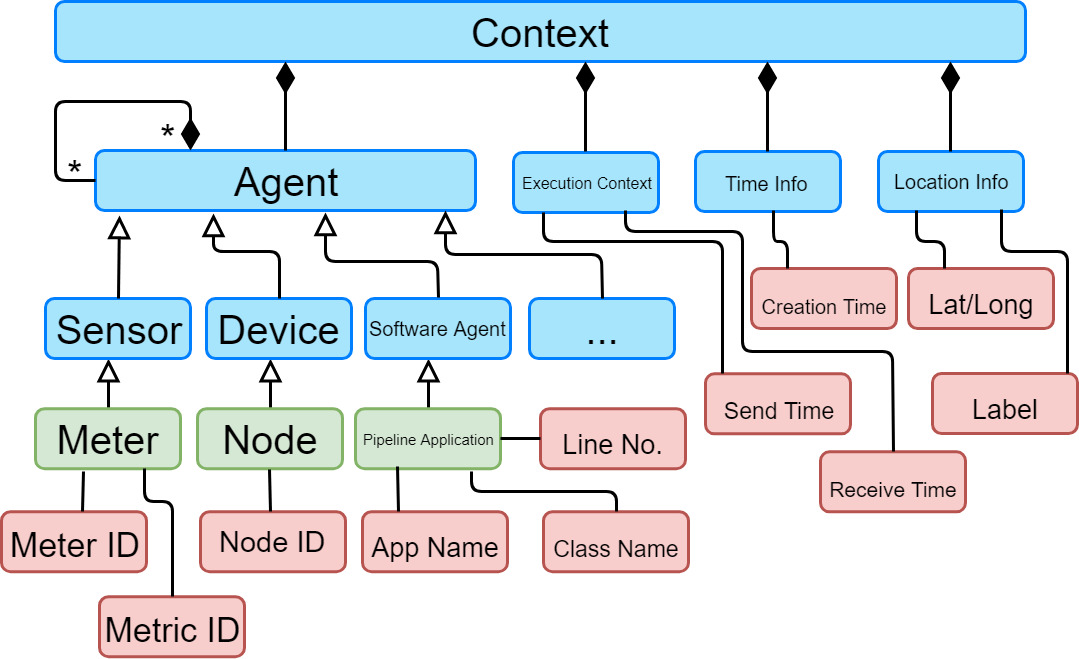
\includegraphics[width=\linewidth]{figures/contextIdp.png}\\
\caption{Use-case specific Data Model Context}
\label{idpDataModelContext}
\end{figure}
We present a visual (cf. \ref{dataModel}) representation of our data model,  where the circle represents a particular provenance data point. The oval inside the circle represents the context in which a particular data value was created and the inner rectangle tells about the set of data values along with the type of transformation/aggregation that caused the creation of new data value. A structured representation (e.g., JSON) is depicted below:

\begin{itemize}			
			\item Example: 
\begin{lstlisting}			
{
    "id": "5a81c0ea00031d239fab",
    "inputDatapoints": [{ 
        "average": [ 
            "5a81c07800031ddaf123",
            "5a81c09300031d341fab"
         ]
    }],
    "context": {
        "loc": {
            "lable": "TU-MAR Building", 
            "latitude": 52.510141,
            "longitude": 13.321451
       },
      "lineNo": 999, "appName": "IDP-App9",
      "className": "MainClass9",
      "timestamp": 1518452970378,
      "sendTime": 1518452970378,
      "receiveTime": 1518452970378,
      "meterId": "2531430010000006834", 
      "metricId": "010151078831",
      "hostId": "239fab"
    } 
}		
\end{lstlisting}

	\end{itemize}
\begin{figure}[h]
\centering
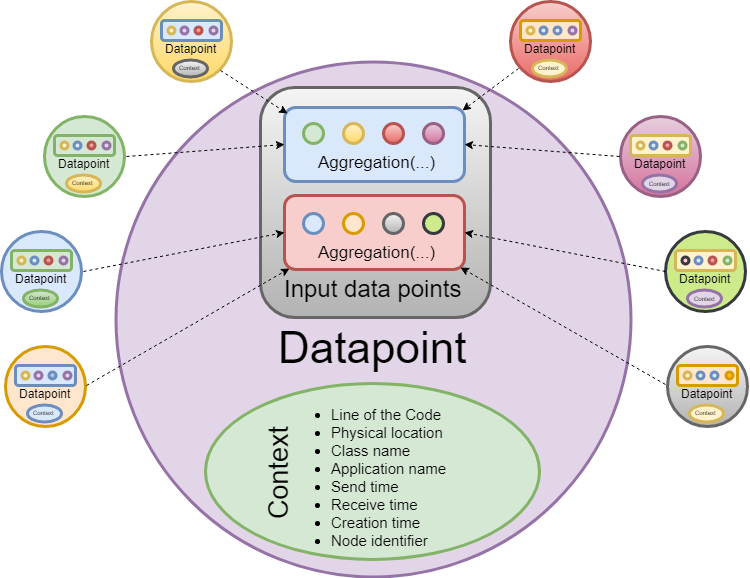
\includegraphics[width=\linewidth]{figures/dataModelforIDP.png}\\
\caption{Data Model}
\label{dataModel}
\end{figure}
\end{itemize}